\section{Highlevel Architecture}
\label{architecture}


\begin{figure}[h]
\begin{center}
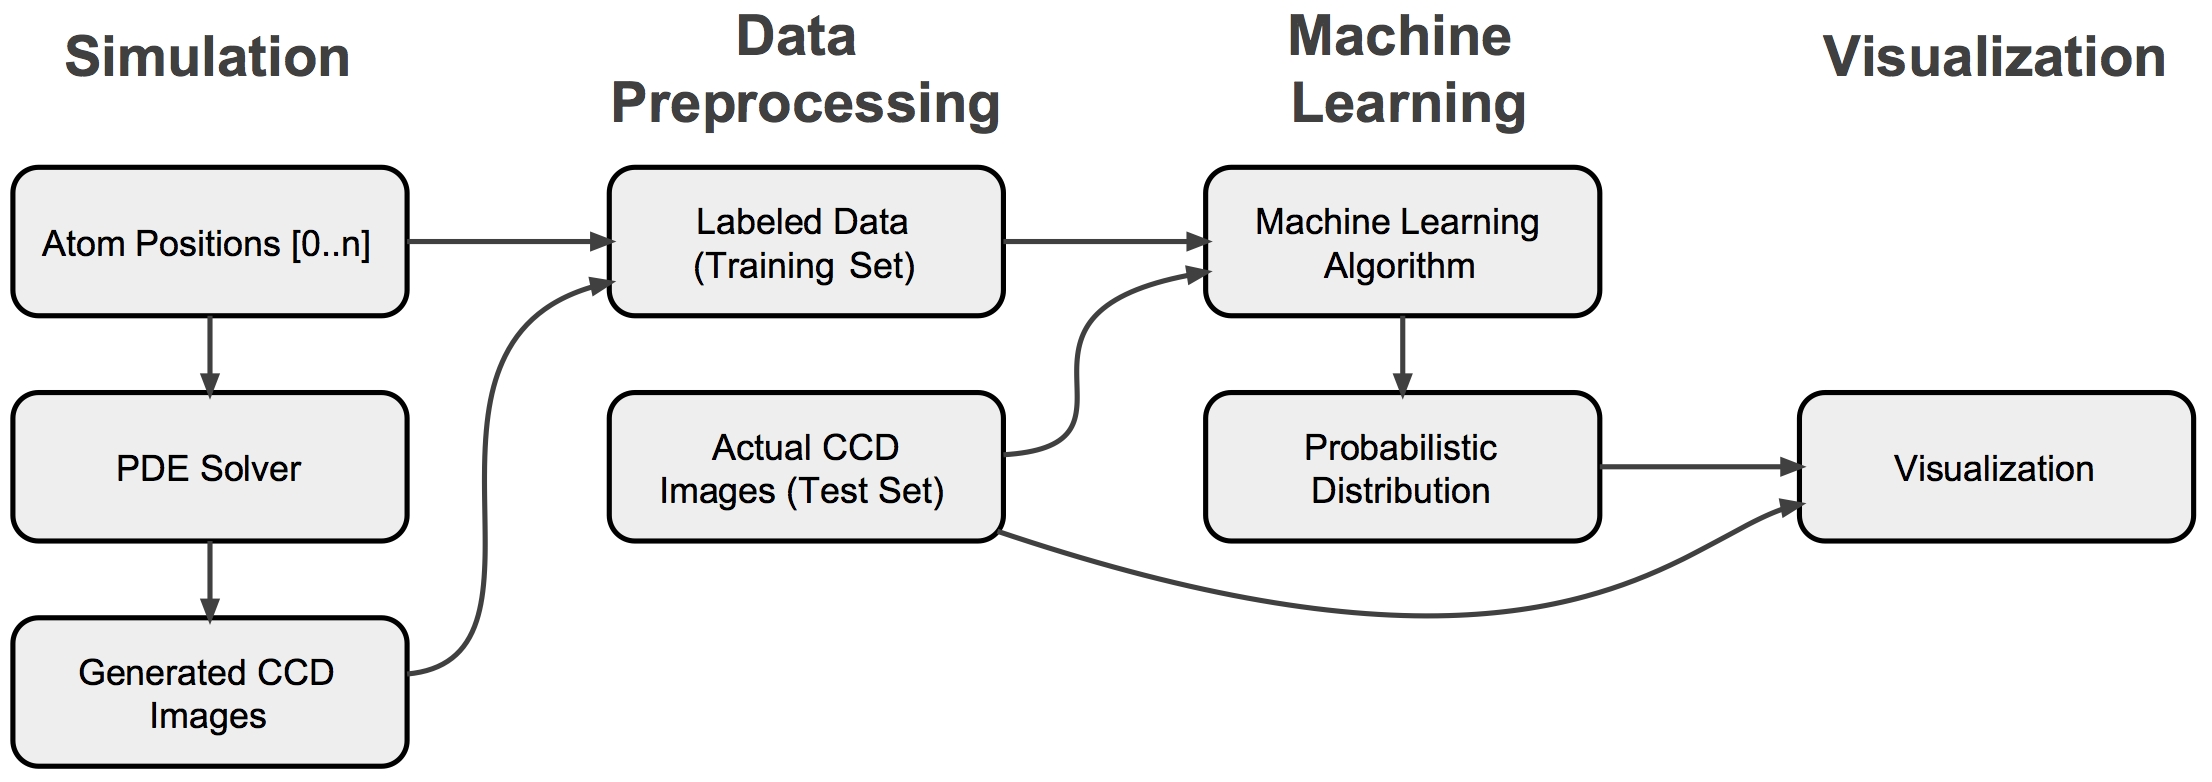
\includegraphics[scale=0.4]{arch.png}
\caption{High Level Architecture Diagram}
\label{fig:arch}
\end{center}
\end{figure}


Figure 1 shows a block level diagram of the AKWDS software (without the visualization component). There are two main programs in the solution.
\begin{description}
\item[AKWDS] This is the control software that OSNAP needs in support of its mission to plan for and execute plans related to real and imagined extraterrestrial encounters. In this case, a hostile invasion scenario.
\item[Simulator] The Simulator is responsible for emulating the world that a deployed AKWDS system would be deployed in. This software supports evaluation and tuning of AKWDS without enduring actual extraterrestrial invasion.
\end{description}
AKWDS and the Simulator will be connected over a network. The Simulator will be responsible for handling the effects of delay called out in the project description.

\subsection{Simulator}
The core of the simulator is a basic physics simulation. This N-body simulation will track projectiles and vehicles within the world and apply basic Newtonian physics. The simulator will expose the current location of each simulated object at regular intervals as a list of 3D cartesian coordinates and object radii. This stream will be sent using the FOSA format. The simulator will also take in a stream of BDS actions and add projectiles to the simulation as appropriate. The simulator also enforces some sanity rules regarding object motion and provides some basic flight paths for UFOs.

\subsection{AKWDS}
AKWDS will take the FOSA stream of object locations and attempt to formulate some tracking of the objects (object A with location $L$ last time step is at location $L'$ this time step). This will be used to help estimate the future location of the object so that targets can be lead correctly for firing. AKWDS will then select a set of object to fire at and set of cannons to fire from and send the needed information via the BDS stream.

\subsection{Visualization}
Visualization is not a core component of the project deliverable. However AKWDS debugging and demonstration will be very difficult without providing some animation of the system behavior. A visualizer, online or post-hoc, that works from the FOSA stream will be provided to help validate the software.